\documentclass{pracamgr}
\usepackage{polski}
\usepackage[utf8]{inputenc}
\usepackage{amssymb}
\usepackage{amsmath}
\usepackage{amsthm}
\usepackage[pdftex]{graphicx}
\usepackage{multicol}
\usepackage{hyperref}

\author{Wiktor Zuba}

\nralbumu{320501}

\title{Efektywne algorytmy generacji obiektów kombinatorycznych???}

\tytulang{Effective algorithms of combinatorial objects generation???}

\kierunek{Informatyka}

\opiekun{prof. Wojciech Rytter\\
Instytut Informatyki}

\date{??? 2017}

\dziedzina{ 
 ???
}


\klasyfikacja{
???
}

\keywords{???}

\newtheorem{defi}{Definicja}[section] %TODO może wprowadzić nową rzecz - oznaczenie np. dla [n], czy u\Delta v
\newtheorem{theorem}{Twierdzenie}
\newtheorem{lemma}[theorem]{Lemat}
\newtheorem{remark}[theorem]{Uwaga}
\newtheorem{fact}[theorem]{Fakt}
\newtheorem{corollary}[theorem]{Wniosek}


\begin{document}
\maketitle

\begin{abstract}
???
\end{abstract}


\tableofcontents%TODO podać, że overline coś to wektor, równy x_1,x_2,...,x_l plus może , overline0 to wektor z samych zer
%TODO wprowadzenie o funkcji Gamma i oszacowaniach na Gamma(k+1/2)/Gamma(k)

 \chapter*{Wprowadzenie}
 \addcontentsline{toc}{chapter}{Wprowadzenie}
  
 \chapter{Własności hiperkostki}
  \section{Podstawowe definicje}
   \begin{defi}\label{[n]}
    Dla $n\in\mathbb{N}$\quad $[n]=\{0,...,n-1\}$ (zbiór pierwszych $n$ liczb naturalnych).
   \end{defi}
   \begin{defi}\label{hiperkostka}
    \emph{Hiperkostką wymiaru $n$ ($Q_n$)} nazwiemy graf, w którym każdy wierzchołek odpowiada ciągowi binarnemu długości $n$,
    zaś krawędzią połączone są te wierzchołki, których ciągi binarne różnią się na dokładnie jednej pozycji.\newline
    $V(Q_n)=\{(v_0,...,v_{n-1}):v_i\in\{0,1\}\}, E(Q_n)=\{(u,v):\sum_{i}|u_i-v_i|=1\}$
   \end{defi}
   \begin{center}
    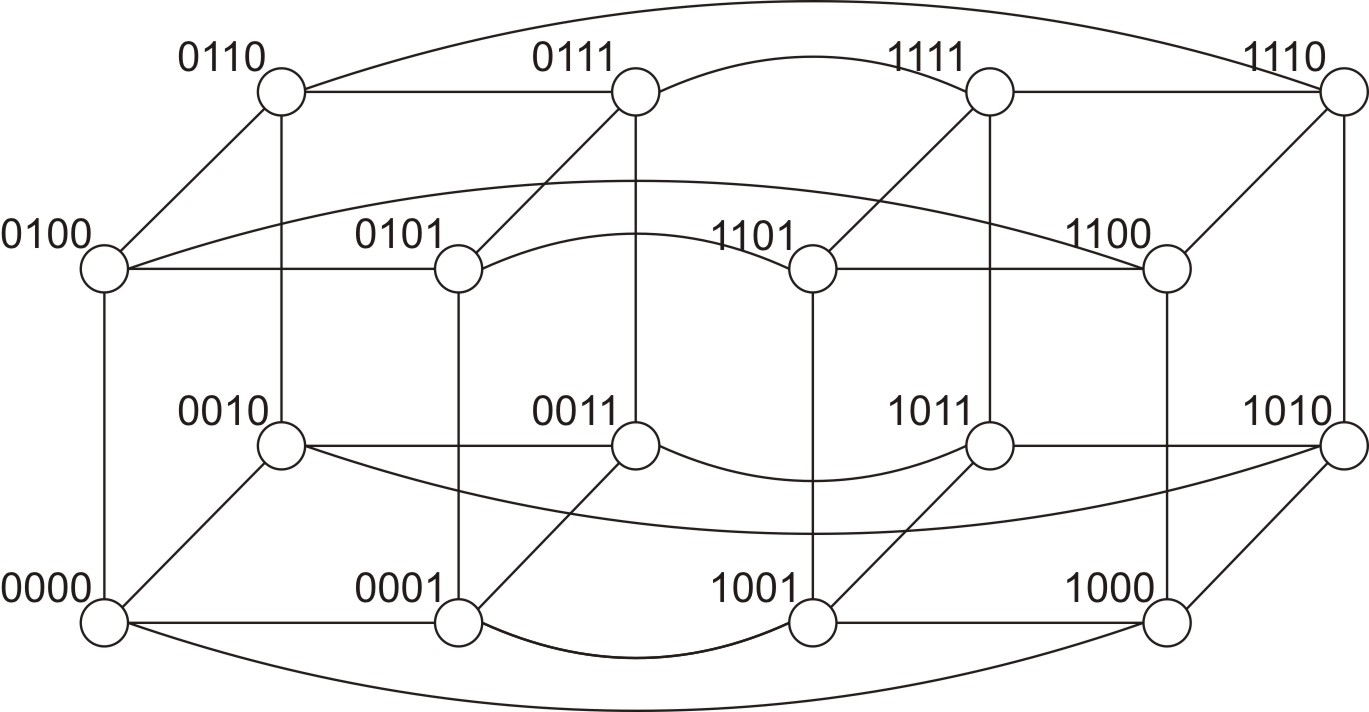
\includegraphics[scale=0.6]{img/Q_4.jpg}
   \end{center}
   W przypadku pełnej hiperkostki %TODO piszę o pełnej, więc trzeba dodać też że są te wadliwe
   bardzo łatwo jest określić długość najkrótszej ścieżki pomiedzy wierzchołkami --
   jest ona równa ilości pozycji na których różnią się ciągi tych wierzchołków.\newline
   Hiperkostka jest grafem dwudzielnym, w którym jedną składową jest zbiór wierzchołków o ciągach z parzystą liczbą jedynek,
   zaś drugą tych o ich nieparzystej liczbie.\newline
   Cowięcej przy badaniu hiperkostek często dzieli się je na $n+1$ warstw, gdzie dla $i\in[n+1]$ $i$-tą warstwę stanowią te wierzchołki,
   których ciągi binarne mają dokładnie $i$ jedynek (warstwa zawiera zatem wierzchołki oddalone o $i$ od wierzchołka zerowego ($\overline{0}$)).
   \begin{defi}\label{delta wierzcholkow}%TODO może do rozdziału o definicjach
    Dla dwóch wierzchołków hiperkostki defininiujemy:
    $u\Delta v=\{i:u_i\neq v_i\}$, gdzie $(u_0,...u_{n-1})$ i $(v_0,...,v_{n-1})$ to ciagi binarne wierzchołków $u$ i $v$ odpowienio
    ($|u\Delta v|$ wyznacza odległość wierzchołków w hiperkostce).
   \end{defi}
   \begin{defi}\label{numerowanie klasyczne}
    \emph{Numerowaniem klasycznym (naturalnym)} hiperkostki nazwiemy takie numerowanie $\varphi:V(Q_n)\rightarrow\{1,...,|V(Q_n)|\}$ jej wierzchołków, że
    $\varphi(v)=1+\sum_{i}v_i\cdot2^i$
   \end{defi}
   \begin{center}
    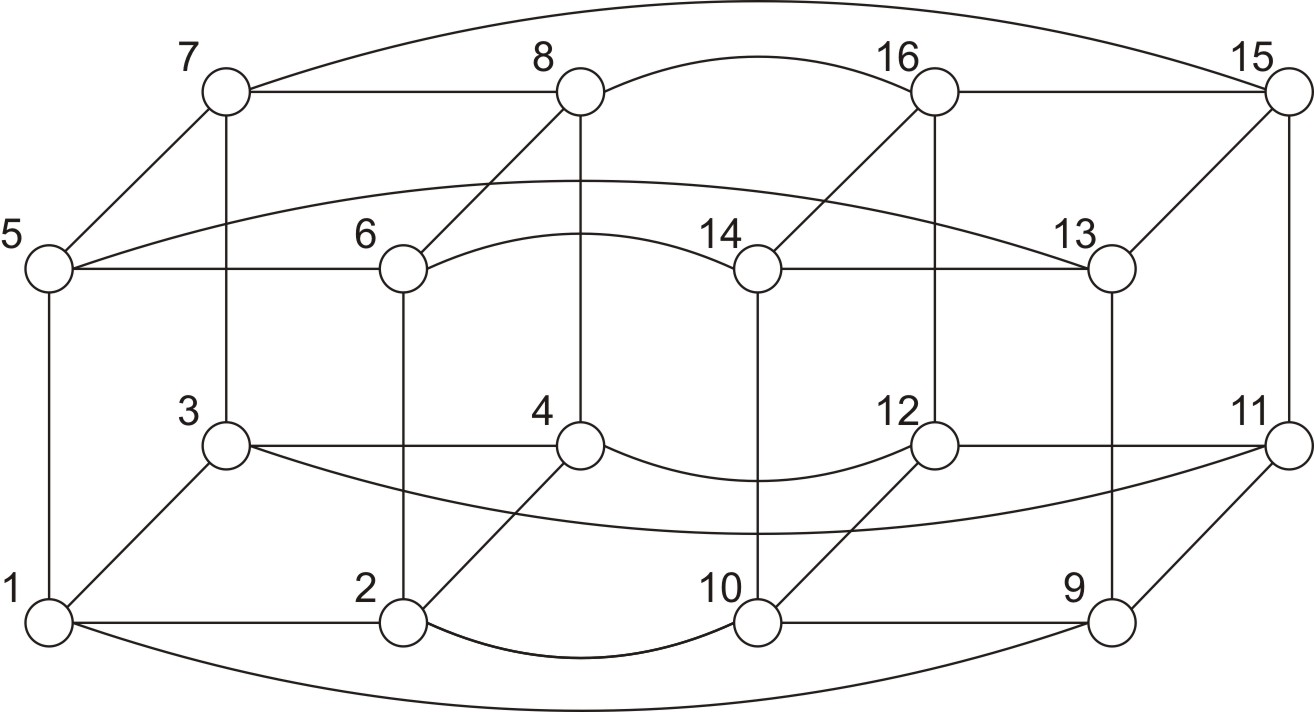
\includegraphics[scale=0.6]{img/Q_4_klasyczne.jpg}
   \end{center}
   \begin{defi}\label{numerowanie warstwowe}%TODO może n choose -1 nie jset tak bardzo standardowe
   \emph{Numerowaniem warstwowym} hiperkostki nazwiemy jej numerowanie w kolejności przeszukiwania grafu wszerz zaczynając od wierzchołka $\overline{0}$
   z wybieraniem sąsiadów w kolejności leksykograficznej.
   \end{defi}
   \begin{center}
    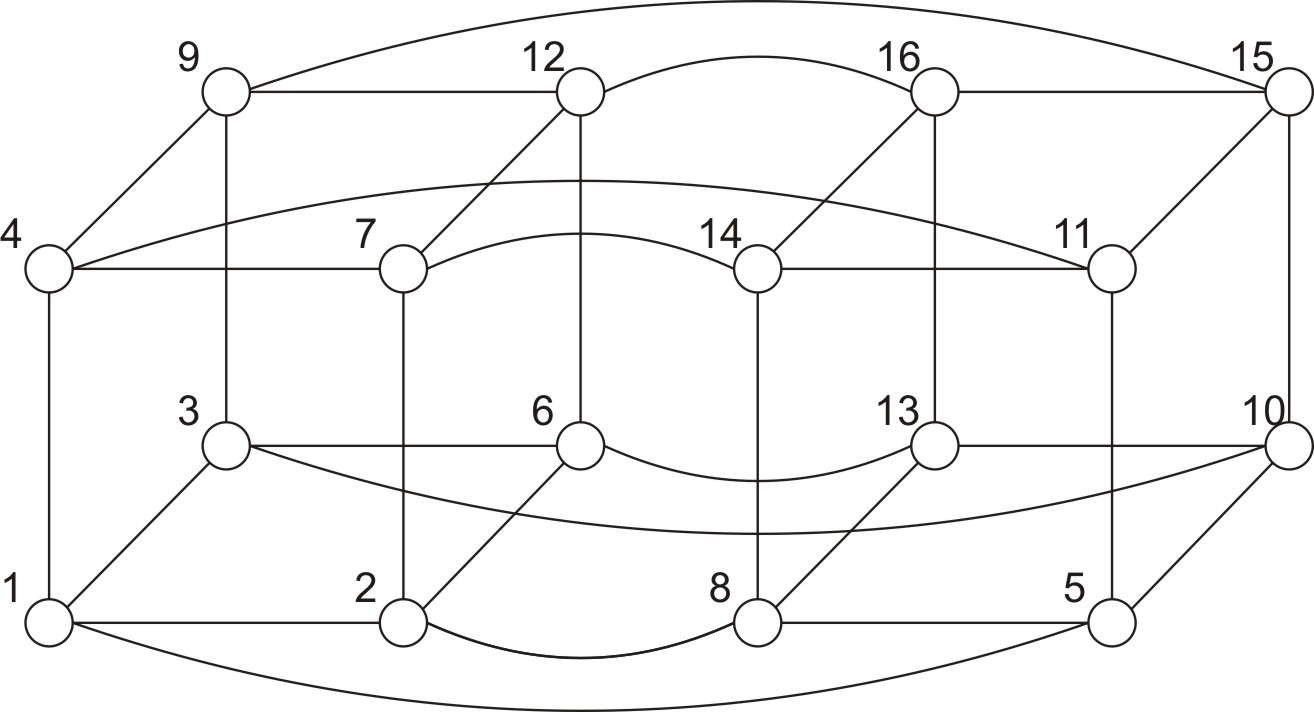
\includegraphics[scale=0.6]{img/Q_4_warstwowe.jpg}
   \end{center}   
   \begin{remark}\label{numerowanie warstwowe 2}
    Jest to takie numerowanie $\varphi:V(Q_n)\rightarrow\{1,...,|V(Q_n)|\}$ jej wierzchołków,
    że wierzchołki z $i$-tej warstwy otrzymują numery od $\sum_{j=0}^{i-1}{n\choose j}+1$ do $\sum_{j=0}^{i}{n\choose j}$.
    W obrębie jednej warstwy numery przyznawane są przeciwnie do kolejności leksykograficznej na odwróconych słowach.
    $\varphi(v)>\varphi(u)\Leftrightarrow (\sum_{i=0}^n v_i>\sum_{i=0}^n u_i)
    \vee((\sum_{i=0}^n v_i=\sum_{i=0}^n u_i)\wedge(\sum_{i=0}^n2^{n-i}v_i<\sum_{i=0}^n2^{n-i}u_i))$
   \end{remark}
   \begin{proof}
    Indukcyjnie po warstwach.\newline
    Dla warstwy $0$ oczywiste.\newline
    Zakładając, że $i$-ta warstwa jest ponumerowana w tym porządku weźmy dwa wierzchołki $u,v$ z warstwy $i+1$:
    $u=(\overline{y_1},1,\overline{x}),v=(\overline{y_2},0,\overline{x})$.\newline
    Jeśli $\overline{y_1}$ zawiera same $0$, to $\overline{y_2}$ zawiera dokładnie jedną $1$, sąsiedzi tych wierzchołków z poprzedniej warstwy
    o namniejszych numerach to odpowiednio $(\overline{0},0,x),(\overline{0},0,x)$,
    tak więc zostaną ponumerowane jako sąsiedzi tego samego wierzchołka, jednak $u$ otrzyma mniejszy numer jako sąsiad mniejszy leksykograficznie.\newline
    Jeśli $\overline{y_1}$ zawiera $1$, to $\overline{y_2}$ też, więc sąsiedzi tych wierzchołków z poprzedniej warstwy
    o namniejszych numerach to odpowiednio $(\overline{y'_1},1,\overline{x}),(\overline{y'_2},0,\overline{x})$, gdzie $\overline{y'_1}$ i $\overline{y'_2}$,
    to odpowiednio $\overline{y_1}$ i $\overline{y_2}$ z pierwszymi $1$ zamienionymi na $0$. Z założenia indukcyjnego sąsiad $u$ ma mniejszy numer niż sąsiad $v$,
    więc $u$ ma mniejszy numer niż $v$.
   \end{proof}
   \begin{defi}\label{sasiedztwo wierzcholka}
    Dla grafu $G$ oraz wierzchołka $v\in V(G)$ definiujemy \emph{sąsiedztwo wierzchołka} jako zbiór wierzchołków połączonych z nim krawędzią:
    $N(v)=\{u\in V(G):(u,v)\in E(G)\}$.
   \end{defi}
   \begin{defi}\label{sasiedztwo zbioru wierzcholkow}%TODO może jakieś lepsze przetłumaczenie boundary
    Dla grafu $G$ oraz zbioru wierzchołków $S\subseteq V(G)$ definiujemy \emph{sąsiedztwo zbioru wierzchołków} jako zbiór tych sąsiadów wierzchołków ze zbioru,
    które same do tego zbioru nie należą: $N(S)=(\bigcup_{v\in S}N(v))\backslash S$
   \end{defi}
   \begin{defi}\label{wnetrze zbioru wierzcholkow}
    Dla grafu $G$ oraz zbioru wierzchołków $S\subseteq V(G)$ definiujemy \emph{wnętrze zbioru wierzchołków} jako zbiór tych wierzchołków z $S$,
    których wszyscy sąsiadzi również należą do tego zbioru: $In(S)=\{v\in S:N(v)\subseteq S\}$
   \end{defi}
   \begin{defi}\label{podgraf indukowany}
    Dla danego $V\subseteq V(G)$\quad $G[V]=(V,\{uv\in E(G):u,v\in V\})$ oznacza \emph{podgraf indukowany} przez podzbiór wierzchołków $V$.
   \end{defi}
   \begin{defi}\label{roznica grafow}
    Dla danego $V\subseteq V(G)$\quad $G-V=G[V(G)\backslash V]$ oznacza \emph{graf $G$ z usuniętymi wierzchołkami $V$}.
   \end{defi}
   \begin{defi}\label{kwadrat grafu}
    Dla danego grafu $G$\newline $G^2=(V(G),E(G)\cup\{uv:\exists_{w\in V(G)}uw\in E(G)\cap wv\in E(G)\})$
    oznacza \emph{kwadrat grafu}, czyli graf z dodanymi krawędziami między wierzchołkami oddalonymi o co najwyżej 2.
   \end{defi}
  \section{Podstawy kombinatoryczne}
   %Wzor Stirlinga: $n!=\sqrt{2\pi n}(\frac{n}{e})^n e^{\lambda_n}$\quad $\frac{1}{12n+1}<\lambda_n<\frac{1}{12n}$\newline
   %${2m \choose m}=\frac{(2m)!}{m!\cdot m!}=
   %\frac{2\sqrt{\pi m}}{2\pi m}\cdot\frac{2^{2m}m^{2m}}{m^{2m}}\cdot\frac{e^{2m}}{e^{2m}}\cdot\frac{e^{\lambda_{2m}}}{e^{2\lambda_m}}=
   %\frac{2^{2m}}{\sqrt{\pi m}}\cdot\frac{e^{\lambda_{2m}}}{e^{2\lambda_m}}$\newline
   %${2m+1 \choose m}={2m+1 \choose m+1}=\frac{(2m+1)(2m)!}{(m+1)m!\cdot m!}=\frac{2m+1}{m+1}\cdot\frac{2^{2m}}{\sqrt{\pi m}}\cdot\frac{e^{\lambda_{2m}}}{e^{2\lambda_m}}$\newline
   %$-\frac{1}{6m}<\frac{-4}{24m+1}<\frac{-3m-1}{m(24m+1)}<\frac{-18m-1}{(24m+1)6m}=\frac{1}{24m+1}-\frac{2}{12m}<\lambda_{2m}-2\lambda_{m}<\frac{1}{24m}-\frac{2}{12m+1}<0$\newline
   %$\frac{1}{\sqrt{m+1}}=\sqrt{m(m+1)}\cdot\frac{1}{(m+1)\sqrt{m}}\le\frac{m+(m+1)}{2}\cdot\frac{1}{(m+1)\sqrt{m}}=\frac{2m+1}{2(m+1)\sqrt{m}}<\frac{1}{\sqrt{m}}$\newline
   %$ 1+\frac{1}{m+1}>e^{\frac{1}{3m}}\Rightarrow e^{-\frac{1}{6m}}>\frac{\sqrt{m+1}}{\sqrt{m+2}}>\frac{\sqrt{m}}{\sqrt{m+1}}$\newline
   %Daje to ograniczenia: $\frac{2^{2m}}{\sqrt{\pi (m+1)}}<{2m \choose m}<\frac{2^{2m}}{\sqrt{\pi m}}$
   %i $\frac{2^{2m+1}}{\sqrt{\pi (m+2)}}<{2m+1 \choose m}={2m+1 \choose m+1}<\frac{2^{2m+1}}{\sqrt{\pi m}}$\newline
   %Lub w krotszym zapisie:
   %$\frac{2^n}{\sqrt{\pi(\lfloor\frac{n}{2}\rfloor}+2)}<{n\choose \lfloor\frac{n}{2}\rfloor}<\frac{2^n}{\sqrt{\pi\cdot\lfloor\frac{n}{2}\rfloor}}$
   ${2n \choose n}=\frac{2^{2n}\Gamma(n+\frac{1}{2})}{\sqrt{\pi}\Gamma(n+1)}$,\quad\quad
   ${2n+1 \choose n}={2n+1 \choose n+1}=\frac{2^{2n+1}\Gamma(n+\frac{3}{2})}{\sqrt{\pi}\Gamma(n+2)}$\newline
   $\Gamma(z)=\int\limits_{0}^{\infty}x^{z-1}e^{-x}dx$\quad
   dla $n\in\mathbb{N}$ $\Gamma(n)=(n-1)!$,\newline
   ogólniej dla $x\in\mathbb{R},x>1$ $\frac{\Gamma(x+1)}{\Gamma(x)}=x$,\quad\quad
   $\frac{\Gamma(x+\frac{1}{2})}{\Gamma(x)}<\frac{\Gamma(x+1)}{\Gamma(x+\frac{1}{2})}\Rightarrow
   \sqrt{x-\frac{1}{2}}<\frac{\Gamma(x+\frac{1}{2})}{\Gamma(x)}<\sqrt{x}$\newline
   Daje to ograniczenia:
   $\frac{2^{2n}}{\sqrt{\pi(n+\frac{1}{2})}}<{2n\choose n}<\frac{2^{2n}}{\sqrt{\pi n}}$,\quad\quad
   $\frac{2^{2n+1}}{\sqrt{\pi(n+\frac{3}{2})}}<{2n+1\choose n}={2n+1\choose n+1}<\frac{2^{2n+1}}{\sqrt{\pi(n+1)}}$\newline
   Lub równoważnie:
   $\frac{2^n}{\sqrt{\pi(\lceil\frac{n}{2}\rceil+\frac{1}{2})}}<{n\choose\lfloor\frac{n}{2}\rfloor}
   ={n\choose\lceil\frac{n}{2}\rceil}<\frac{2^n}{\sqrt{\pi\lceil\frac{n}{2}\rceil}}$
   \begin{lemma}\label{binomial sum upper bound}
    Dla $k\le\lfloor\frac{n+1}{2}\rfloor$ zachodzi ograniczenie $\sum_{i=0}^{k-1}{n\choose i}\le2^{n-1}\frac{{n\choose k}}{{n\choose \lfloor\frac{n}{2}\rfloor}}$
   \end{lemma}
   \begin{proof}
    (Uogólnienie dowodu z podobnego lematu dla $n=2m,k<m$ z \cite{LPV})\newline% Lemma3.8.2
    Załóżmy najpierw, że $k<\lfloor\frac{n}{2}\rfloor$\newline
    Zdefiniujmy $c=\frac{{n\choose k}}{{n\choose \lfloor\frac{n}{2}\rfloor}}<1,t=\lfloor\frac{n}{2}\rfloor-k,$
    $A=\sum_{i=0}^{k-1}{n\choose i}, B=\sum_{i=k}^{\lfloor\frac{n}{2}\rfloor-1}{n\choose i}$\newline
    $\forall_{1\le i\le k}$ $\frac{{n\choose k-i}}{{n\choose \lfloor\frac{n}{2}\rfloor-i}}<\frac{{n\choose k-i+1}}{{n\choose \lfloor\frac{n}{2}\rfloor-i+1}}$
    $\Leftrightarrow \frac{k-c+1}{n-k+c}<\frac{\lfloor\frac{n}{2}\rfloor-c+1}{\lceil\frac{n}{2}\rceil+c}$,\newline
    co wynika z szeregu prostych nierówności $\frac{k-c+1}{n-k+c}\le\frac{k-c+1}{k+c+1}
    <\frac{\lfloor\frac{n}{2}\rfloor-c+1}{\lfloor\frac{n}{2}\rfloor+c+1}\le\frac{\lfloor\frac{n}{2}\rfloor-c+1}{\lceil\frac{n}{2}\rceil+c}$)\newline
    Daje nam to ograniczenia $\forall_{1\le i\le k}$ $\frac{{n\choose k-i}}{{n\choose \lfloor\frac{n}{2}\rfloor-i}}<c$.\newline
    Suma ostatnich $t$ wyrazów szeregu $A$ jest majoryzowana przez $c\cdot B$, wcześniejszych $t$ przez $c$ razy suma ostatnich $t$ (a więc przez $c^2\cdot B$).
    Daje nam to oszacowanie $A<(c+c^2+c^3+...+c^{\lfloor\frac{k}{t}\rfloor})\cdot B<(c+c^2+c^3+...)\cdot B=\frac{c}{1-c}\cdot B$.
    Jednocześnie $A+B=\sum_{i=0}^{\lfloor\frac{n}{2}\rfloor-1}{n\choose i}<2^{n-1}$.
    $A=c\cdot A+(1-c)\cdot A=c(A+\frac{1-c}{c}A)<c\cdot(A+B)<c\cdot 2^{n-1}$.\newline
    Pozostaje udowodnić przypadki większych $k$:\newline
    Dla $n=2m,k=m$ $\sum_{i=0}^{m-1}{2m\choose i}=2^{2m-1}-\frac{1}{2}{2m\choose m}<2^{2m-1}=
    2^{n-1}\cdot\frac{{n\choose k}}{{n\choose \lfloor\frac{n}{2}\rfloor}}$\newline
    Dla $n=2m+1,k=m$ $\sum_{i=0}^{m-1}{2m+1\choose i}=2^{2m}-{2m+1\choose m}<2^{2m}=
    2^{n-1}\cdot\frac{{n\choose k}}{{n\choose \lfloor\frac{n}{2}\rfloor}}$\newline
    Dla $n=2m+1,k=m+1$ $\sum_{i=0}^{m}{2m+1\choose i}=2^{2m}=
    2^{n-1}\cdot\frac{{n\choose k}}{{n\choose \lfloor\frac{n}{2}\rfloor}}$ (jedyna nieostra nierówność)\newline
   \end{proof}
  \section{Własność ekspansji}
   \begin{defi}\label{epsilon ekspansja wierzcholkowa}
    Graf $G$ posiada własność \emph{$\varepsilon$--ekspansji wierzchołkowej}, jeżeli dla każdego zbioru wierzchołków $S\subseteq V(G)$ takiego,
    że $|S|\le\frac{|V(G)|}{2}$ zachodzi $|N(S)|\ge\varepsilon\cdot|S|$
   \end{defi}
   \begin{lemma}
    Zbiór pierwszych $l$ wierzchołków hiperkostki według numerowania warstwowego posiada maksymalne wnętrze wśród zbiorów wielkości $l$.  
   \end{lemma}\label{HAR1}
   Jest to jeden z lematów dowodzonych w pracy \cite{HAR}.
   \begin{lemma}\label{S->S_k}%TODO chyba niezdefionowane S_k
    Dla hiperkostki do udowodnienia własności $\varepsilon_n$--ekspansji wierzchołkowej wystarczy rozważyć zbiory $S$ postaci $S_k,k\le 2^{n-1}$.
   \end{lemma}
   \begin{proof}
    Weżmy dowolne $S\subseteq V(G), l=|S|+|N(S)|$ z Lematu \ref{HAR1} wynika, że
    $\frac{|N(S)|}{|S|}=\frac{|N(S)|+|S|}{|S|}-1\ge\frac{|S_l|}{|In(S_l)|}-1=\frac{|S_l\backslash In(S_l)|}{|In(S_l)|}\ge\frac{|N(In(S_l))|}{|In(S_l)|}$.
    Z definicji $S_l$ wynika, że $In(S_l)=S_k$ dla $k=In(S_l)$.\newline
    Pozostaje udowodnić, że wystarczy rozważyć te $S_k$, że $k\le2^{n-1}$\newline
    Dla $l=|N(S)|+|S|\ge(\varepsilon_n+1)\cdot 2^{n-1}$ mamy $|S|>2^{n-1}$ lub $|N(S)|\ge\varepsilon_n|S|$, wystarczy więc rozważyć przypadek
    $l<(\varepsilon_n+1)\cdot 2^{n-1}$.\newline
    Dla $n=2m+1$ weżmy $k=2^{n-1}=\sum_{i=0}^{m}{2m+1 \choose i}$, wtedy $S_k$ = pełne $m+1$ pierwszych warstw i $N(S_k)$ = warstwa $m+1$.
    Przykład ten pokazuje, że $\varepsilon_n\le\frac{{2m+1 \choose m+1}}{2^{2m}}$,
    więc $l<2^{2m}+{2m+1 \choose m+1}\Rightarrow$ $S_l$ mieści się w piewszych $m+2$ warstwach
    $\Rightarrow$ $S_k=In(S_l)$ mieści się w pierwszych $m+1$ warstwach $\Rightarrow k\le 2^{2m}=2^{n-1}$.\newline
    Dla $n=2m$ weżmy $k=2^{n-1}=\sum_{i=0}^{m-1}{2m \choose i}+\frac{1}{2}{2m\choose m}$, wtedy $S_k$ = pełne $m$ pierwszych warstw + połowa środkowej.
    W środkowej warstwie pierwsze ${2m-1\choose m-1}=\frac{1}{2}{2m \choose m}$ wierzchołków to dokładnie te, których ciągi binarne kończą się na $1$.
    Wtedy też $S_k\cup N(S_k)$ to dokłanie pełne $m+1$ pierwszych warstw plus te wierzchołki z warstwy $m+2$, które kończą się na $1$
    $\Rightarrow |N(S_k)|={2m-1\choose m}+{2m-1\choose m}={2m-1\choose m-1}+{2m-1 \choose m}={2m\choose m}$.
    Przykład ten pokazuje, że $\varepsilon_n\le\frac{{2m \choose m}}{2^{2m-1}}$,
    więc $l<2^{2m-1}+{2m \choose m}\Rightarrow$ $S_l$ mieści się w piewszych $m+1$ warstwach plus tych wierzchołkach z warstwy $m+2$, które kończą się na $1$
    $\Rightarrow k\le2^{n-1}$.
   \end{proof}
   \begin{corollary}\label{ograniczenie ekspansji}
    Hiperkostka wymiaru $n$ nie posiada własności $\frac{2\sqrt{2}}{\sqrt{\pi n}}$--ekspansji wierzchołkowej.
   \end{corollary}
   \begin{proof}%TODO mozna by wylaczyc te gamma stad do tego podrozdzialu o kombinatrycznych
    Dla $n=2m+1$\newline
    $\frac{|N(S_{2^{2m}})|}{|S_{2^{2m}}|}=\frac{{2m+1 \choose m+1}}{2^{2m}}=\frac{2^{2m+1}}{2^{2m}\sqrt{\pi(m+1)}}=\frac{2}{\sqrt{\pi(m+1)}}=
    \frac{2}{\sqrt{\pi(\frac{n}{2}+\frac{1}{2})}}=\frac{2\sqrt{2}}{\sqrt{\pi(n+1)}}<\frac{2\sqrt{2}}{\sqrt{\pi n}}$.\newline
    Dla $n=2m$
    $\frac{|N(S_{2^{2m-1}})|}{|S_{2^{2m-1}}|}=\frac{{2m \choose m}}{2^{2m-1}}<\frac{2^{2m}}{2^{2m-1}\sqrt{\pi(m+1)}}=\frac{2}{\sqrt{\pi m}}=
    \frac{2}{\sqrt{\pi\cdot\frac{n}{2}}}=\frac{2\sqrt{2}}{\sqrt{\pi n}}$.
   \end{proof}
   \begin{theorem}\label{ekspansja kostki}%TODO spróować wzmocnić do \frac{2}{\sqrt{\pi n}}
    Hiperkostka $Q_n$ posiada własność $\frac{1}{\sqrt{\pi n}}$--ekspansji wierzchołkowej.
   \end{theorem}
   \begin{proof}
    Jeśli $k=\sum_{i=0}^{r}{n\choose i}$ (pełne $r+1\le\lfloor\frac{n}{2}\rfloor+1$ warstw), to%TODO podać oszacowanie na sum {n\choose i}
    $\frac{|N(S_k)|}{|S_k|}=\frac{{n\choose r+1}}{\sum_{i=0}^{r}{n \choose i}}>\frac{{n\choose r+1}{n\choose \lfloor\frac{n}{2}\rfloor}}{2^{n-1}{n\choose r+1}}
    =\frac{{n\choose \lfloor\frac{n}{2}\rfloor}}{2^{n-1}}>\frac{2^{n}}{2^{n-1}\sqrt{\pi (\lceil\frac{n}{2}\rceil+\frac{1}{2})}}=
    \frac{2}{\sqrt{\pi (\lceil\frac{n}{2}\rceil+\frac{1}{2})}}
    \ge\frac{2\sqrt{2}}{\sqrt{\pi (n+\frac{3}{2})}}\ge\frac{2}{\sqrt{\pi n}}$ (dla $n\ge2$).\newline
    ($n=2m+1,r=m$ rozważone w \ref{S->S_k})\newline
    Jeśli $k=\sum_{i=0}^{r}{n\choose i}+{n-1 \choose r}$
    (pełne $r+1\le\lfloor\frac{n}{2}\rfloor+1$ warstw ? TODO + te wierzchołki z warstwy $r+2$, których ciągi binarne kończą się na $1$).\newline
    $|N(S_k)\cup S_k|=\sum_{i=0}^{r+1}{n\choose i}+{n-1 \choose r+1}\Rightarrow |N(S_k)|=2\cdot{n-1\choose r+1}$\newline
    $\frac{|N(S_k)|}{|S_k|}=\frac{2\cdot{n-1 \choose r+1}}{\sum_{i=0}^{r}{n\choose i}+{n-1 \choose r}}>
    \frac{2\cdot{n-1\choose r+1}{n\choose\lfloor\frac{n}{2}\rfloor}}{2^{n-1}\cdot{n\choose r+1}+{n-1\choose r}\cdot{n\choose\lfloor\frac{n}{2}\rfloor}}=
    \frac{2\cdot{n-1\choose r+1}{n\choose\lfloor\frac{n}{2}\rfloor}}{2^{n-1}\cdot({n-1\choose r}+{n-1\choose r+1})+{n-1\choose r}\cdot{n\choose\lfloor\frac{n}{2}\rfloor}}>\newline
    \frac{2\cdot{n-1\choose r+1}{n\choose\lfloor\frac{n}{2}\rfloor}}{2^{n}\cdot{n-1\choose r+1}+{n-1\choose r}\cdot{n\choose\lfloor\frac{n}{2}\rfloor}}=
    \left(\frac{2^{n-1}}{{n\choose\lfloor\frac{n}{2}\rfloor}}+\frac{{n-1\choose r}}{2\cdot{n-1\choose r+1}}\right)^{-1}>
    \left(\frac{\sqrt{\pi(n+\frac{3}{2})}}{2\sqrt{2}}+\frac{1}{2}\right)^{-1}=\frac{2\sqrt{2}}{\sqrt{\pi(n+\frac{3}{2})}+\sqrt{2}}>\frac{2}{\sqrt{\pi n}}$ (dla $n\ge 7$).\newline
    W pozostałych przypadkach można otrzymać ograniczenie choć dużo gorsze wiedząc, że dodanie wierzchołka do $S$ zmniejszy $N(S)$ o co najwyżej $1$.\newline
    Weźmy teraz $\sum_{i=0}^{r}{n\choose i}<k<\sum_{i=0}^{r}{n\choose i}+{n-1 \choose r}$\newline
    $\frac{|N(S_k)|}{|S_k|}>\frac{{n\choose r+1}-{n-1\choose r}}{\sum_{i=0}^{r}{n\choose i}+{n-1 \choose r}}=
    \frac{{n-1\choose r+1}}{\sum_{i=0}^{r}{n\choose i}+{n-1 \choose r}}\ge
    \frac{\frac{1}{2}{n \choose r+1}}{\sum_{i=0}^{r}{n\choose i}+\frac{1}{2}{n \choose r+1}}
    \left(\frac{\sqrt{\pi (n+\frac{3}{2})}}{\sqrt{2}}+1\right)^{-1}>\frac{1}{\sqrt{\pi n}}$ (dla $n\ge 7$).\newline
    Analogicznie da $\sum_{i=0}^{r}{n\choose i}+{n-1 \choose r}<k<\sum_{i=0}^{r+1}{n\choose i}$\newline
    $\frac{|N(S_k)|}{|S_k|}>\frac{2{n-1\choose r+1}-{n-1\choose r+1}}{\sum_{i=0}^{r+1}{n\choose i}}=
    \frac{{n-1\choose r+1}}{\sum_{i=0}^{r+1}{n\choose i}}>
    \frac{{n-1\choose r+1}}{2^{n-1}\frac{{n\choose r+1}}{{n\choose\lfloor\frac{n}{2}\rfloor}}+{n\choose r+1}}\ge
    \frac{{n\choose r+1}{n\choose\lfloor\frac{n}{2}\rfloor}}{(2^{n-1}+{n\choose\lfloor\frac{n}{2}\rfloor}){n\choose r+1}}=
    \frac{{n\choose\lfloor\frac{n}{2}\rfloor}}{2^{n-1}+{n\choose\lfloor\frac{n}{2}\rfloor}}>
    \left(\frac{\sqrt{\pi (n+\frac{3}{2})}}{\sqrt{2}}+1\right)^{-1}>\frac{1}{\sqrt{\pi n}}$ (dla $n\ge 7$).\newline
    Dla przypadków $n\le6$ można ręcznie sprawdzić wszystkie $2^{n-1}$ przypadków, aby również otrzymać oszacowanie $\frac{1}{\sqrt{\pi n}}$.
   \end{proof}
 \chapter{Problemy na wadliwej hiperkostce}
  \section{Graf z wadami}
   \begin{defi}\label{graf z wadami}
    W grafie $G$ możemy wyróżnić niektóre wierzchołki (czasem również krawędzie) i oznaczyć jako wadliwe.
    Graf z niepustym takim wyróżnionym zbiorem wierzchołków wadliwych $F\subseteq V(G)$ nazywamy \emph{grafem z wadami} (lub \emph{grafem wadliwym})
   \end{defi}%TODO może dodać wspomnienie, że wadliwy też nazywany usuniętym
    Wadliwe wierzchołki (i/lub krawędzie) najczęściej traktowane są jako usunięte z grafu -- mówimy w tym przypadku o grafie $G-F$.
    Wyróżnianie wadliwych wierzchołków w grafie zamiast definiowania nowego grafu jest umotywowane głównie w przypadkach,
    gdy pełny graf łatwo zdefiniować i zapisać w pamięci małej względem jego rozmiaru (np. klika, hiperkostka, graf de Bruijna),
    a zbiór wadliwych wierzchołków jest również mały.
  \section{Spójność wadliwej hiperkostki}
   \textbf{Ten podrozdział jest napisany w większości na podstawie \cite{DFGKR}.}
   \begin{remark}\label{spojnosc przy usunietych}
    Aby zbadać spójność grafu $G-F$ dla spójnego grafu $G$ wystarczy sprawdzić czy wciąż istnieje ścieżka pomiędzy dowolnymi dwoma wierzchołkami,
    które oryginalnym grafie sąsiadowały z jakimś spośród usuniętych wierzchołków (wszystkie takie wierzchołki należą do jedenj spójnej składowej).
   \end{remark}
   \begin{proof}
    Aby udowodnić spójność trzeba pokazać, że istnieje ścieżka pomiędzy dowolnymi dwoma wierzchołkami, jednak skoro w oryginalnym grafie taka ścieżka istniała,
    to w nowym grafie jedyną przeszkodą jest to, że na tej ścieżce mogły występować wierzchołki, które zostały usunięte. Taką scieżkę można naprawić wstawiając
    w miejsca od pierwszego do ostatniego wystąpienia wierzchołka usuniętego ścieżkę pomiędzy odpowiednimi ich sąsiadami istniejącą w pomniejszonym grafie.
   \end{proof}
   \subsection{Podejście ekspansywne}\label{podejscie ekspansywne}
    \begin{theorem}\label{Spójność ekspansywna}
     Niech graf $G$ posiada własność $\varepsilon$--ekspansji wierzchołkowej z $\varepsilon>0$ i maksymalny stopień wierzchołka $\Delta$,
     oraz dana jest wyrocznia zwracająca dla danego wierzchołka listę jego sąsiadów.
     Wtedy istnieje algorytm, który otrzymuje na wejściu zbiór $F\subseteq V(G)$ oraz $\varepsilon$
     i testuje spójność $G-F$ w czasie $O\left(\frac{|F|^2\cdot\Delta^2\cdot\log(|V(G)|)}{\varepsilon}\right)$
    \end{theorem}
    \begin{lemma}\label{klasyfikacja skladowych}
     Spójna składowa $S\subseteq V(G)\backslash F$ grafu $G-F$ jest jednego z dwóch typów:
     \begin{itemize}
      \item główna -- $|S|>\frac{|V(G)|}{2}$
      \item mała -- $|S|\le\frac{|F|}{\varepsilon}$
     \end{itemize}
    \end{lemma}
    \begin{remark}\label{klasyfikacja skladowych 2}
     Co prawda dla dużego $|F|$ i małego $\varepsilon$ może być tak, że składowa jest jednocześnie główna i mała, jednak po pierwsze jest to przypadek mało
     interesujacy, gdyż wtedy zwykłe przeszukiwanie grafu spełnia tezę twierdzenia, a po drugie przypadek ten nie psuje w żaden sposób otrzymywanego algorytmu.
     W lemacie istotne jest to, że w grafie nie ma składowych średnich wielkości.
    \end{remark}
    \begin{fact}\label{jedna glowna skladowa}
     Może być tylko jedna składowa główna.
    \end{fact}
    \begin{proof}
     (Lematu)\newline
     Weźmy spójną składową $S$ grafu $G-F$ ($N_{G-F}(S)=0$), jeżeli $S\le\frac{|V(G)|}{2}$, to z własności $\varepsilon$--ekspansji wierzchołkowej grafu $G$
     $|N_G(S)|\ge\varepsilon\cdot|S|$ (gdzie $S$ jest teraz traktowane jako podzbiór wierzchołków grafu $G$). Gdyby zachodziło $|S|>\frac{|F|}{\varepsilon}$,
     to mielibyśmy $|N_G(S)|>\frac{\varepsilon\cdot|F|}{\varepsilon}=|F|$, co daje sprzeczność ponieważ aby w grafie $G-F$ to sąsiedztwo było puste z grafu
     $G$ trzeba usunąć co najmniej $N_G(S)$ wierzchołków.
    \end{proof}
    \begin{proof}
     (Twierdzenia)\newline
     Chcemy sprawdzić, czy wszyscy sąsiedzi wierzchołków usuniętych należą do tej samej spójnej składowej. Na podstawie lematu \ref{klasyfikacja skladowych},
     jeśli składowa zawierająca taki wierzchołek jest większa niż $\frac{|F|}{\varepsilon}$, to jest to składowa główna.
     Jeżeli wszystkie takie wierzchołki spełniają ten warunek, to $G-F$ jest spójny.
     Jeżeli natomiast, któraś z tych składowych okaże się mała, to $G-F$ nie jest spójny.\newline
     Wystarczy więc uruchomić liniowe przeszukiwanie grafowe w każdym wierzchołku sąsiadującym z wierzchołkiem wadliwym i przerywać po przejrzeniu
     $\frac{|F|}{\varepsilon}$ wierzchołków.\newline
     Algorytm liniowego przeszukiwania grafowego uruchamiany jest co najwyżej $|F|\cdot\Delta$ razy.
     Za każdym razem przeglądamy co najwyżej $\frac{|F|}{\varepsilon}$ wierzchołków.
     Dla każdego przeglądanego wierzchołka sprawdzamy co najwyżej $\Delta$ sąsiadów, a odpowiedź wyroczni zajmuje $O(log(|V(G)|))$ czasu.
     Daje to złożoność z tezy twierdzenia.
    \end{proof}
    \begin{corollary}\label{ekspansywna spojnosc dla kostki}
     Ponieważ zgodnie z twierdzeniem \ref{ekspansja kostki} hiperkostka $Q_n$ posiada własność\newline
     $\frac{1}{\sqrt{\pi n}}$--ekspansji wierzchołkowej,
     oraz można znaleźć wszystkich sąsiadów wierzchołka w czasie liniowym od ich ilości powyższy algorytm testuje spójność wadliwej hiperkostki w czasie
     ${O(|F|^2\cdot n^{3.5})}$ (wyrażonego w ilości operacji arytmetycznych).
    \end{corollary}
    \begin{remark}\label{prawdziwa zlozoność ekspansywnej}
     Ze względu na długość zapisu identyfikatora wierzchołka liniową od wymiaru hiperkostki nie da się przeprowadzać operacji na wierzchołkach w czasie szybszym niż
     $n$. To dolne ograniczenie jest osiągalne przy przechowywaniu przejrzanych wierzchołków w hashmapie
     (czas oczekiwany operacji $O(n)$, złożoność pamięciowa całej struktury $O(n^{0.5}|F|)$),
     lub w drzewie prefiksowym (czas pesymistyczny operacji $O(n)$, złożoność pamięciowa całej struktury $O(n^{1.5}|F|)$).
     Pozwala to w łatwy sposób uzyskać efektywną wyrocznię, a więc i algorytm o złożoności z wniosku.
    \end{remark}
    TODO pseudokod
   \subsection{Redukcja przy pomocy transformacji ścieżek}
    Algorytm przedstawiony w poprzednim podrozdziale jest dowodem na to, że testowanie spójności wadliwej hiperkostki może być zrobione wielomianowo
    ze względu na ilość wad i wymiar hiperkostki. Algorytm ten wykorzystuje jednak bardzo płytko potencjał tak regularnego grafu.
    W tym podrozdziale przedstawię algorytm, który dzięki głębszemu wykorzystaniu własności hiperkostki otrzymuje lepsze rezultaty złożonościowe.
    \begin{defi}\label{podgrafy kostki}
     Na potrzeby tego podrozdziału definiuję ze pracą \cite{DFGKR} dla $F\subseteq V(Q_n)$\newline
     podgraf $G(F)=(A\cup B\cup F,E)$ grafu $Q_n$,
     gdzie $A=N(F),\quad B=N(A)\backslash F,\newline E=\{uv\in E(Q_n):u\in A\cup F\}$ (podgraf zawierający wierzchołki w odległości $\le 2$ od wierzchołków wadliwych,
     plus krawędzie w których jeden z końców jest wadliwy lub z takim sąsiaduje).
    \end{defi}
    \begin{theorem}\label{spojnosc z lokalnej spojnosci}
     Dla $F\subseteq V(Q_n)$ graf $Q_n-F$ jest spójny wtedy i tylko wtedy gdy dla każdej $C$ -- spójnej składowej $Q_n^2[F]$ spójny jest graf $G(C)-C$.
    \end{theorem}
    \subsubsection{Transformacje ścieżek w hiperkostce}
     \begin{defi}\label{sekwencja tranzycji}
      Dla ścieżki $W=(v_0,v_1,...,v_n)$ (z możliwymi powtórzeniami) w hiperkostce \emph{sekwencją tranzycji} nazywamy ciąg $\tau=(d_1,d_2,...,d_n)$,
      gdzie $d_i$ jest współrzędną na której różnią się ciągi binarne wierzchołków $v_{i-1}$ i $v_i$.
     \end{defi}
     \begin{fact}\label{sekwencja tranzycji - parzystość}%TODO trzeba wprowadzić [n]
      $\tau$ jest sekwencją tranzycji pewnej $uv$--ścieżki w $Q_n$ wtedy i tylko gdy\newline
      $u\Delta v=\{i\in[n]:\#(\tau,i)$ nieparzyste$\}$,
      gdzie $\#(\tau,i)$ to ilość wystąpień $i$ w sekwencji $\tau$.
     \end{fact}
     Dla $\tau$ -- sekwencji tranzycji $uv$--ścieżki $W$ definiujemy trzy operacje:
     \begin{itemize}
      \item $swap(\tau_1,i,j,\tau_2)=(\tau_1,j,i,\tau_2)$\quad dla $\tau=(\tau_1,i,j,\tau_2)$
      \item $insert_i(\tau_1,\tau_2)=(\tau_1,i,i,\tau_2)$\quad dla $\tau=(\tau_1,\tau_2),i\in[n]$
      \item $delete(\tau_1,i,i,\tau_2)=(\tau_1,\tau_2)$\quad dla $\tau=(\tau_1,i,i,\tau_2)$
     \end{itemize}
     Wszystkie te operacje nie zmieniają parzystości wystąpień współrzędnych, dlatego też dowolnie w ten sposób zmodyfikowana sekwencja
     wciąż jest sekwencją tranzycji pewnej $uv$--ścieżki w $Q_n$.
     \begin{defi}\label{sciezki rownowazne}
      Dwie ścieżki, których sekwencje tranzycji $\tau,\rho$ spełniają $\forall_{i\in[n]}\#(\tau,i)=\#(\rho,i)$ nazywamy \emph{równoważnymi}.
     \end{defi}
     \begin{remark}\label{przeksztalcanie sciezek}
      Dla dowolnych dwóch $uv$--ścieżek w $Q_n$ istnieje sekwencja operacji $swap,insert,delete$ (w tej kolejności bez przeplotów),
      która przemiania sekwencję tranzycji pierwszej w sekwencję tranzycji drugiej.
     \end{remark}
     \begin{proof}
      Jeśli dwie ścieżki są równoważne, to można jedną przekształcić w drugą przy pomocy samych operacji $swap$.\newline
      W przypadku gdy sekwencje mają różne liczności wystąpień współrzędnych, to można je doprowadzić do takich $\tau',\rho'$,
      że $\forall_{i\in[n]}\#(\tau',i)=\#(\rho',i)$ przy pomocy samych operacji $insert$ (używanych w dowolnie wybranych wierzchołkach).
     \end{proof}
     \begin{defi}\label{port}
      Na potrzeby dowodu twierdzenia \ref{spojnosc z lokalnej spojnosci} dla $uv$--ścieżki $W=(w_0,w_1,...,w_k)$ (gdzie $w_0=u,w_k=v$) wierzchołek
      $w_i$ nazywamy portem, jeśli nie jest wierzchołkiem wadliwym, ale dokładnie jeden z jego sąsiadów w ścieżce należy do $F$ (port musi więc należeć do $A$).
     \end{defi}
     W przypadku tej definicji należy rozróżnić przeplatające się pojęcia wierzchołka grafu i jego wystąpienia na ścieżce --
     portem nazywane jest konkretne wystąpienie na ścieżce, inne jego wystąpienia nie muszą być portami.\newline
     Dla $C$ spójnej składowej $G(F)-F$ przez $p(C,W)$ oznaczamy ilość portów w części $W$ nalezącej do $C$.
     \begin{lemma}\label{parzystosc portow swap}
      Operacja swap zachowuje parzystość $p(C,W)$.
     \end{lemma}
     \begin{proof}
      Dowód stanowi rysunkowe rozpatrzenie wszystkich możliwych przypadków w których w wyniku operacji $swap$ powstaje i/lub znika pewien port
      (przypadki przy końcach ścieżki można "dopełnić" zwykłymi wierzchołkami do przypadków ze środka ponieważ wierzchołki końcowe nie są wadliwe).
      \begin{multicols}{3}
       \begin{center}
        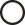
\includegraphics[scale=1]{img/Q_swap_l1.jpg}
        -- wierzchołek zwykły\newline
        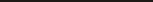
\includegraphics[scale=1]{img/Q_swap_l4.jpg}
        -- krawędź ścieżki\newline
       \end{center}
       \begin{center}
        
\includegraphics[scale=1]{img/Q_swap_l2.jpg}
        -- wierzchołek wadliwy\newline
        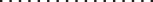
\includegraphics[scale=1]{img/Q_swap_l5.jpg}
        -- krawędź spoza ścieżki\newline
       \end{center}
       \begin{center}
        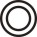
\includegraphics[scale=1]{img/Q_swap_l3.jpg}
        -- port\newline
        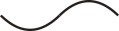
\includegraphics[scale=1]{img/Q_swap_l6.jpg}
        -- nieistotna reszta ścieżki\newline
       \end{center}
      \end{multicols}
      \noindent
      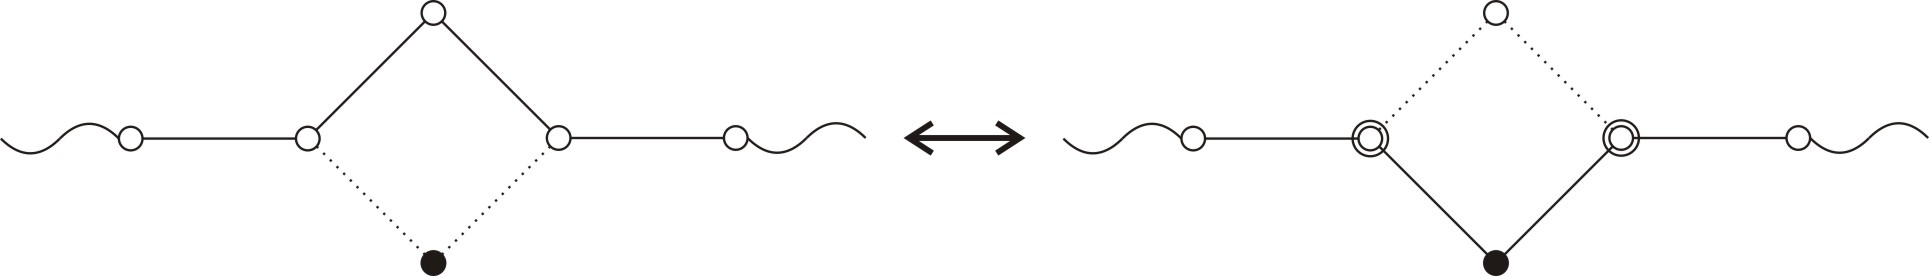
\includegraphics[scale=1]{img/Q_swap_1.jpg}\newline\newline
      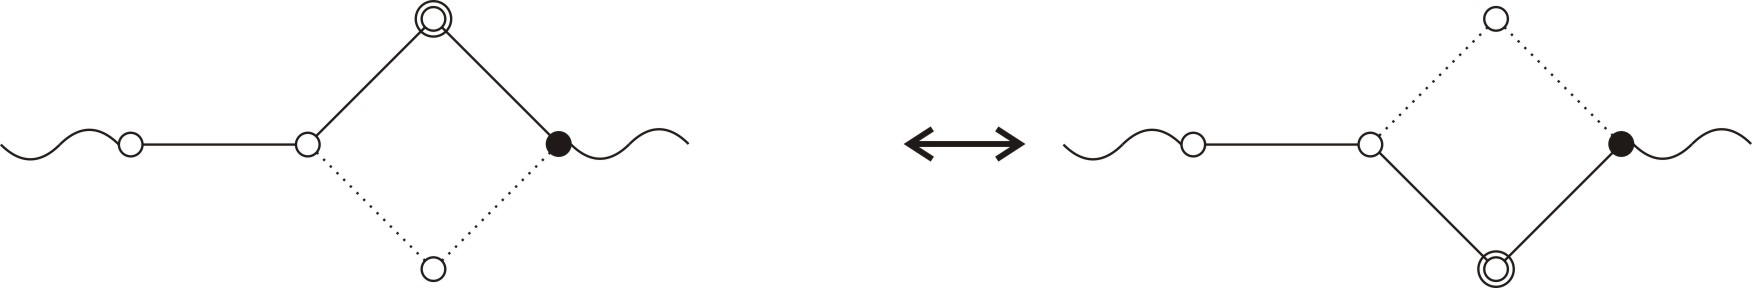
\includegraphics[scale=1]{img/Q_swap_2.jpg}\newline\newline
      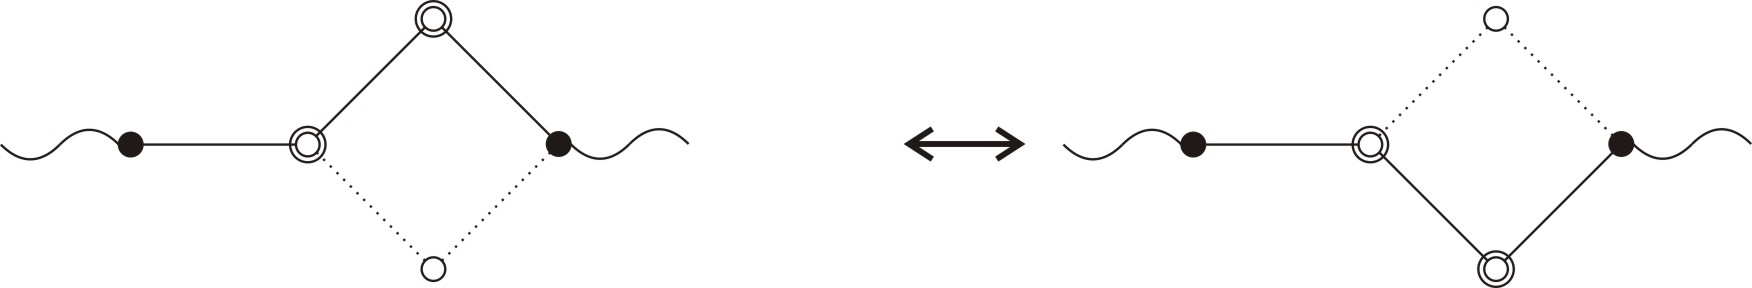
\includegraphics[scale=1]{img/Q_swap_3.jpg}\newline\newline
      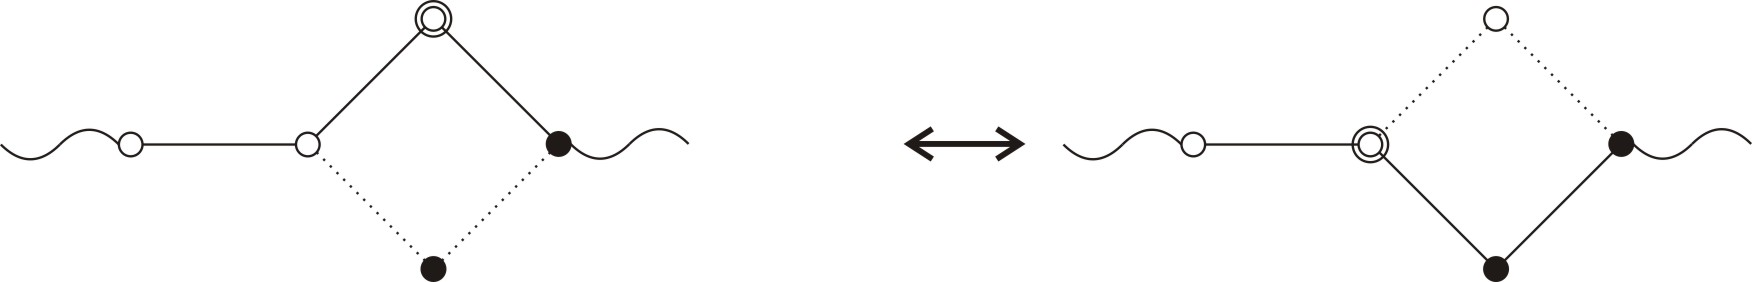
\includegraphics[scale=1]{img/Q_swap_4.jpg}\newline\newline
      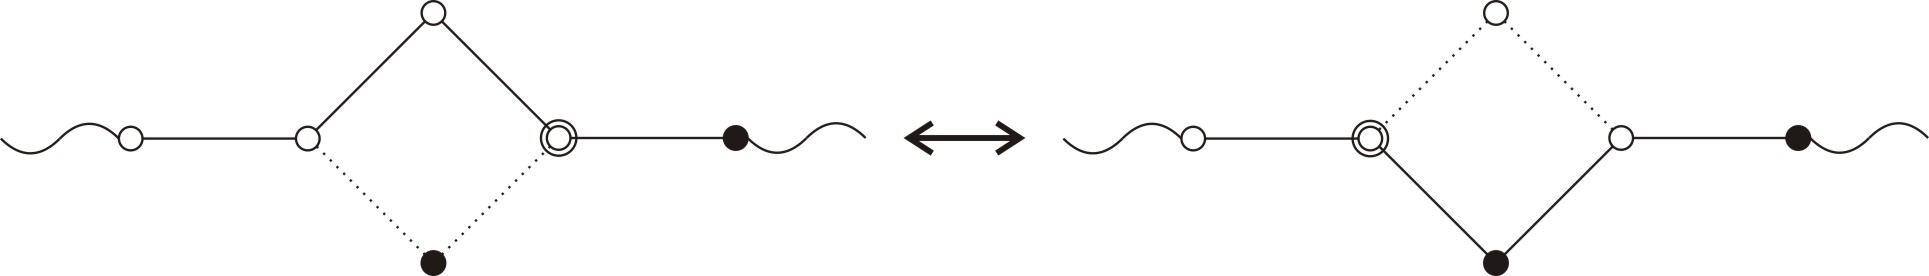
\includegraphics[scale=1]{img/Q_swap_5.jpg}\newline\newline
      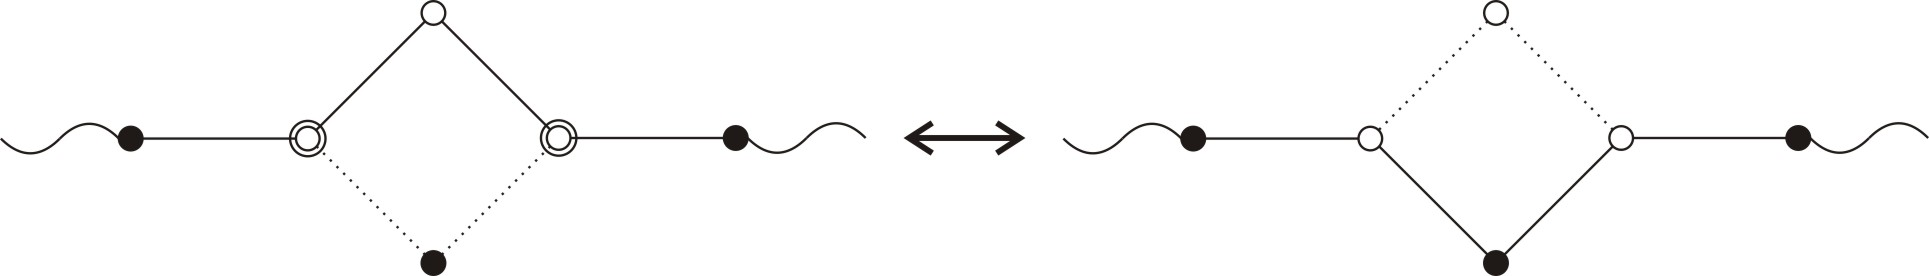
\includegraphics[scale=1]{img/Q_swap_6.jpg}\newline\newline
      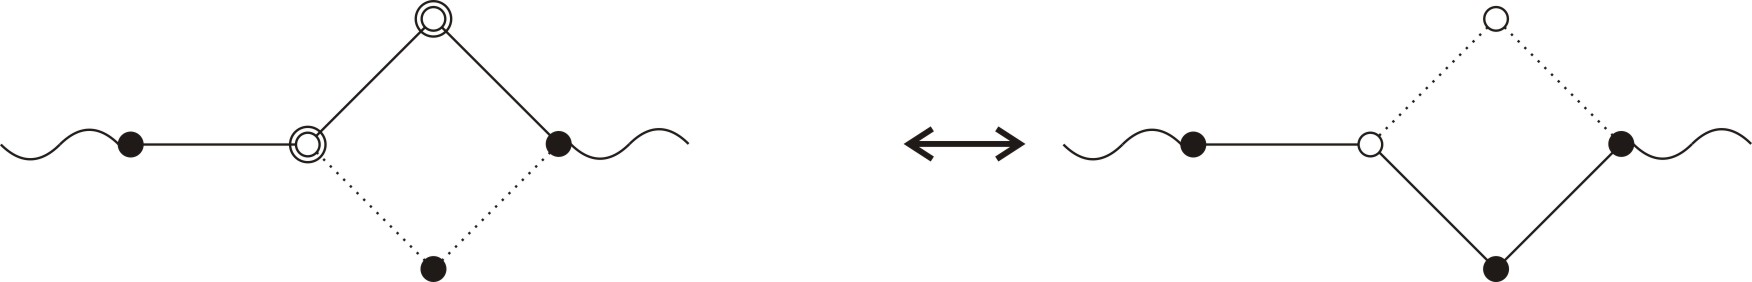
\includegraphics[scale=1]{img/Q_swap_7.jpg}\newline\newline
      Wszystkie rozrysowane tu wierzchołki należą do $G(F)$, a rozrysowane części niewadliwe tworzą podgraf spójny, dlatego też wszystkie te zmiany odbywają się w
      jednej spójnej składowej $G(F)-F$. Za każdym razem ilość portów zmienia się o $0$ lub $2$, a więc parzystość pozostaje bez zmian.
     \end{proof}
    \subsubsection{Dowód twierdzenia o lokalnej spójności}
     \begin{lemma}\label{Q_n-F spojne => G(F)-F spojne (1 skladowa)}
      Niech $F\subseteq V(Q_n)$ takie, że $G(F)$ jest spójne. Jeśli $Q_n-F$ jest spójne, to $G(F)-F$ również.
     \end{lemma}
     \begin{proof}
      Załóżmy przeciwnie -- istnieją wierzchołki $u,v\in A\cup B=V(G(F)-F)$ dla których istnieje ścieżka $P$ w $Q_n-F$, ale nie ma takiej w  $G(F)-F$.
      Skoro w $G(F)-F$ nie ma takiej ściezki, to w $P$ musi występować wierzchołek $x$ spoza $A\cup B$.\newline
      $G(F)$ jest spójne, więc musi istnieć też druga ścieżka $R$ łacząca $u$ z $v$ w tym właśnie grafie, na której występuje wierzchołek $y\in F$.\newline
      Podobnie jak w dowodzie lematu \ref{przeksztalcanie sciezek} 
      ścieżki te mogą być napompowane w wierzchokach $x$ i $y$ odpowidnio sekwencjami operacji $insert$.\newline
      Ponieważ $x$ jest oddalone od $F$ dodane do ścieżki $P$ wierzchołki nie uczynią z zadnego wystąpienia $x$ portu i same również nie staną się portami.
      Ponieważ $y$ należy do $F$ dodane do ścieżki $R$ wierzchołki będą miały dokładnie dwóch sąsiadów z $F$ (tego samego dwukrotnie), a więc nie będą portami.\newline
      Oznacza to, że uzyskane ścieżki równoważne mają tyle samo portów we wszystkich spójnych składowych $G(F)-F$ co odpowiadające im nieprzekształcone
      a na podstawie lematów \ref{przeksztalcanie sciezek} i \ref{parzystosc portow swap} ich parzystości między sobą się zgadzają (czyli zgadzają się dla $P$ i $R$).
      Na ścieżce $P$ nie ma żadnych portów ponieważ nie występuje w niej żaden wierzchołek wadliwy,
      daje to sprzeczność ponieważ dla spójnych składowych $G(F)-F$ w której występują
      $u$ i $v$ ścieżka $R$ ma nieparzyste ilości portów (np. można dobrać taką ścieżkę, która wchodzi do/opuszcza składowe co najwyżej raz).
     \end{proof}
     \begin{corollary}\label{Q_n-F spojne => Q_n^2[F]-F spojne (1 skladowa)}
      Dla $F\subseteq V(Q_n)$ takiego, że $Q_n^2[F]$ jest spójne ze spójności $Q_n-F$ wynika spójność $G(F)-F$.
     \end{corollary}
     \begin{proof}
      Jeśli dwa wierzchołki $Q_n^2[F]$ są połączone, to w oryginalnym grafie musiały być w odległości $\le 2$, a więc w $G(F)$ muszą być połączone
      albo bezpośrednio albo poprzez pojedynczy wierzchołek z $A$, a więc graf $G(F)$ jest spójny co sprawia,
      że spełnione są założenia lematu.
     \end{proof}
     \begin{lemma}\label{Q_n^2[F]-F spojne => Q_n-F spojne}
      Niech $F\subseteq V(Q_n)$ taki, że $G(C)-C$ jest spójne dla kazdej $C$ spójnej składowej $Q_n^2[F]$. Wtedy $Q_n-F$ również jest spójny.
     \end{lemma}
     \begin{proof}
      Dla dowolnie wybranych dwóch wierzchołków $u,v\in V(Q_n-F)$ weźmy $W$ -- ścieżkę między nimi w pełnym $Q_n$. Jeśli $W$ nie zawiera wadliwego wierzchołka,
      to jest poprawną ścieżką w $Q_n-F$. W przeciwnym przypadku znajdujemy na tej ścieżce pierwsze wystąpienie wierzchołka wadliwego.
      Poprzedni wierzchołek na ścieżce oraz pierwszy kolejny z poza zbioru $F$ są dwoma niewadliwymi wierzchołkami należącymi do $G(C)$, gdzie $C$
      jest spójną składową $Q_n^2[F]$ (oddalone o 1 od wadliwych wierzchołków, które są połączone ścieżką samych wadliwych wierzchołków).
      W $G(C)$ nie ma wadliwych wierzchołków spoza $C$, ponieważ oznaczałoby to, że taki wierzchołek jest oddalony o $\le 2$ od pewnego wierzchołka z $C$,
      a więc byłby z nim połączony w $Q_n^2$, dlatego też ścieżka ze spójnego z założenia $G(C)-C$ nie zawiera wadliwego wierzchołka.
      Wystarczy więc wadliwą część ścieżki $W$ zastąpić odpowiednią ścieżką z $G(C)-C$ aby otrzymać poprawną ścieżkę w $Q_n-F$.
     \end{proof}
     \begin{proof}
      (Twierdzenia \ref{spojnosc z lokalnej spojnosci})\newline
      Lemat \ref{Q_n^2[F]-F spojne => Q_n-F spojne} jest implikacją w jedną stronę.
      W drugą stronę dla spójnego $Q_n^2[F]$ jest dana wnioskiem \ref{Q_n-F spojne => Q_n^2[F]-F spojne (1 skladowa)}.
      Wystarczy udowodnić, że nic nie psuje się w przypadku gdy $Q_n^2[F]$ ma więcej niż jedną spójną składową.
      Dla $C$ -- spójnej składowej $Q_n^2[F]$ jeśli $Q_n-F$ jest spójne, to jest takie również $Q_n-C$
      (dla wierzchołków spoza $Q_n-F$ te same ścieżki są dobre, dla tych z  $F\backslash C$ dowolny sąsiad nalezy do $Q_n-F$, więc również łatwo zbudować ścieżkę),
      a więc spójne jest również $G(C)-C$ co kończy dowód.
     \end{proof}
    \subsubsection{Algorytm}
     Stosując powyższe twierdzenie można uzyskać wielomianowy algorytm uzywając jedynie przeszukiwania grafowego
     podobnie jak w podrozdziale \ref{podejscie ekspansywne}. Można jednak uzyskać lepsze rezultaty używając dodatkowo struktury $Find$--$Union$ i sprawdzając
     spójności już w trakcie budowania podgrafów $G(C)-C$.\newline
     W algorytmie używane są:
     \begin{itemize}
      \item struktura $Find$--$Union$ $D$ z operacjami:
       \begin{itemize}
        \item $Make(v,D)$ tworzącą singleton $\{v\}$
        \item $Find(v,D)$ zwracającą wskaźnik na zbiór zawierający $v$
        \item $Union(u,v,D)$ łączącą zbior zawierający $u$ ze zbiorem zawierającym $v$
       \end{itemize}
       których zamortyzowany czas można ograniczyć przez $O(log m)$ (a da się nawet uzyskać $O(log^*m)$), gdzie $m$ jest ilością użyć
       operacji $Make(v,D)$.
       Dodatkowo struktura zapewnia możliwość sprawdzenia, czy zawiera więcej niż jeden zbiór (wystarczy pojedynczy licznik inkrementowany przy
       $Make(v,D)$ i dekrementowany przy $Union(u,v,D)$).
      \item strukturę $T$ do przechowywania informacji o niektórych wierzchołkach jak binarne drzewo prefiksowe lub hashmapa,
       przechowywującą dla wierzchołka $v_T$ informacje:
       \begin{itemize}
        \item wskaźnik do wierzchołka $v$ w strukturze $D$
        \item informacje o wadliwości/braku wadliwości wierzchołka
        \item binarną informacje o tym czy wierzchołek był odwiedzony i należy do $F\cup N(F)$
       \end{itemize}
       wspierającą operacje:
       \begin{itemize}
        \item $Insert(v,T)$ wstawiającą wierzchołek $v$ do struktury $T$ i zwracającą wskaźnik na $v_T$
        \item $Retrieve(v,T)$ zwracającą $v_T$ lub $NULL$ w przypadku gdy $v$ nie ma w strukturze
       \end{itemize}
       które wymagają $O(n)$ czasu na wykonanie.
     \end{itemize}
     
     Definiuję pomocniczą funkcję uzyskiwania wierzchołków ze struktury $T$ i inicjalizowania w razie nieobecności:\newline\newline
     \hspace*{0pt}$Retrieve2(v,T)\{$\newline
     \hspace*{16pt}	$v_T=Retrieve(v,T);$\newline
     \hspace*{16pt}	if$(v_T==NULL)\{$\newline
     \hspace*{32pt}		$v_T=Insert(v,T);$\newline
     \hspace*{32pt}		$v_T.healthy=TRUE;$\newline
     \hspace*{32pt}		$v_T.visited=FALSE;$\newline
     \hspace*{32pt}		$Make(v,D);$\newline
     \hspace*{16pt}	$\}$\newline
     \hspace*{16pt}	return$(v_T);$\newline
     \hspace*{0pt}$\}$\newline
     
     Najistotniejszą częścią algorytmu jest procedura (czasami dla wielu wierzchołków z $F$) $DFS(f)$ znajdująca spójne składowe $G(C)-C$,
     dla $C$ spójnej składowej $Q_n^2[F]$ zawierającej wadliwy wierzchołek $f$, o następującym pseudokodzie:\newline\newline    
     \hspace*{0pt}$DFS(f)\{$\newline
     \hspace*{16pt}	foreach$(u\in N(f))\{$\newline
     \hspace*{32pt}		$u_T=Retrieve2(u,T);$\newline
     \hspace*{32pt}		if$(u_T.visited==FALSE)\{$\newline
     \hspace*{48pt}			$u_T.visited=TRUE;$\newline
     \hspace*{48pt}			if$(u_T.healthy)\{$\newline
     \hspace*{64pt}				foreach$(v\in N(u))\{$\newline
     \hspace*{80pt}					$v_T=Retrieve2(v,T);$\newline
     \hspace*{80pt}					if$(v_T.healthy)\{$\newline
     \hspace*{96pt}						if$(Find(u,D)\neq Find(v,D))\quad\backslash\backslash$ krawędź $uv$ należy do $G(C)-C$\newline
     \hspace*{80pt}					$\}$else if$(v_T.visited==FALSE)\{$\newline
     \hspace*{96pt}						$v_T.visited=TRUE;$\newline
     \hspace*{96pt}						$DFS(v);\quad\backslash\backslash$ wadliwy wierzchołek należący do $C$\newline
     \hspace*{80pt}					$\}$\newline
     \hspace*{64pt}				$\}$\newline
     \hspace*{48pt}			$\}$else$\quad DFS(u);\quad\backslash\backslash$ wadliwy wierzchołek należący do $C$\newline
     \hspace*{32pt}		$\}$\newline
     \hspace*{16pt}	$\}$\newline
     \hspace*{0pt}$\}$\newline
     
     Powyższa prodedura uruchamiana jest z funkcji głównej:\newline\newline
     \hspace*{0pt}$Conectivity(n,F)\{$\newline
     \hspace*{16pt}	$T=empty\_structureT();$\newline
     \hspace*{16pt}	foreach$(f\in F)\{$\newline
     \hspace*{32pt}		$f_T=Insert(f,T);$\newline
     \hspace*{32pt}		$f_T.healthy=FALSE;$\newline
     \hspace*{32pt}		$f_T.visited=FALSE;$\newline
     \hspace*{16pt}	$\}$\newline
     \hspace*{16pt}	foreach$(f\in F)\{$\newline
     \hspace*{32pt}		$f_T=Retrieve(f,T);$\newline
     \hspace*{32pt}		if$(f_T.visited==FALSE)\{$\newline
     \hspace*{48pt}		$f_T.visited=TRUE;$\newline
     \hspace*{48pt}		$D=empty\_structureD();$\newline
     \hspace*{48pt}		$DFS(f);$\newline
     \hspace*{48pt}		if$(D.counter>1)\quad return(FALSE);$\newline
     \hspace*{32pt}		$\}$\newline
     \hspace*{16pt}	$\}$\newline
     \hspace*{16pt}	$return(TRUE);$\newline
     \hspace*{0pt}$\}$
    \subsubsection{Analiza złożoności}
    
     
\begin{thebibliography}{99}%TODO dziwne litery , upcase?
\addcontentsline{toc}{chapter}{Bibliografia}

  \bibitem{LPV} L. Lovasz, J. Pelikan and K. Vesztergombi.
   "Discrete Mathematics, Elementary and Beyond."
   \textit{Undergraduate Texts in Mathematics. New York: Springer, first edition, 2003}   

  \bibitem{HAR} L. H. HARPER,
   "Optimal Numberings and Isoperimetric Problems on Graphs"
   \textit{JOURNAL OF COMBINATORIAL THEORY 1, 385-393 (1966)}
   
  \bibitem{DFGKR} Tomas Dvorak, Jirı Fink, Petr Gregor, Vaclav Koubek and Tomasz Radzik,
   "Efficient connectivity testing of hypercubic networks with faults"
   
   %------------------------------------------------------------pompowanie   
  \bibitem{FG} Jirı Fink and Petr Gregor,
   "Long paths and cycles in hypercubes with faulty vertices"
   
  \bibitem{FG2} Jirı Fink and Petr Gregor,
   "Long pairs of paths in faulty hypercubes"
   
  \bibitem{HHH} Frank Harary, John P. Hayes and Horng--Jyh Wu,
   "A survey of theory of hypercube graphs"
   \textit{Comput. Math. Applic. Vol. 15, No 4, pp. 277-289, 1988}
   
  \bibitem{HL} Frank Harary, Marilynn Livingston,
   "Independent domination in hypercubes"
   \textit{Appl. Math. Lett. Vol. 6, No 3, pp. 27-28, 1993}
   
  \bibitem{RS} Wojciech Rytter $\&$ Bartosz Szreder,
   "Wprowadzenie do kombinatoryki algorytmicznej"
   
  \bibitem{Knuth} DONALD E. KNUTH,
   "Generating All Tuples and Permutations"
   \textit{THE ART OF COMPUTER PROGRAMMING VOLUME 4, FASCICLE 2}
  
  \bibitem{Ruskey} FRANK RUSKEY,
   "Combinatorial Generation"
   \textit{Working Version, October 1, 2003}

  \bibitem{SW} Tibor Szabo, Emo Weltz,
   "Unique Sink Orientations of Cubes"
   
  \bibitem{Wong} Chi Him Wong,
   "Novel universal cycle constructions for a variety of combinatorial objects"
   \textit{Guelph, Ontario, Canada, April, 2015}
   
\end{thebibliography}

\end{document}